\documentclass{article}
\usepackage[utf8]{inputenc}
\usepackage[spanish]{babel}
\usepackage[margin=0.9in]{geometry}
\usepackage{graphicx}
\usepackage{subfigure}
\usepackage{float}
\usepackage{amsmath}
\usepackage{listings}
\usepackage{color}

\definecolor{dkgreen}{rgb}{0,0.6,0}
\definecolor{gray}{rgb}{0.5,0.5,0.5}
\definecolor{mauve}{rgb}{0.58,0,0.82}

\lstset{frame=tb,
  language=Python,
  aboveskip=3mm,
  belowskip=3mm,
  showstringspaces=false,
  columns=flexible,
  basicstyle={\small\ttfamily},
  numbers=left,
  numberstyle=\tiny\color{gray},
  keywordstyle=\color{blue},
  commentstyle=\color{dkgreen},
  stringstyle=\color{mauve},
  breaklines=true,
  breakatwhitespace=true,
  tabsize=3
}

\title{Informe de la Tarea Investigativa II, presentado por los estudiantes del equipo No.-27}
\author{Raudel Alejandro G\'omez Molina - 211 \\ Fernando Vald\'es Garc\'ia - 212}
\date{}

\begin{document}

    \maketitle

    \begin{center}
        
        \LARGE{\textbf{Stability analysis of an SIR model with immunity and modified transmission function}} \par \bigskip
        \normalsize
        \Large{\textbf{Nidhi Nirwani, V.H.Badshah, R.Khandelwal}}  \\ \bigskip
        \textbf{International Journal of Applied Mathematical Research, 2015}
        Factor de impacto: 0.55 
    \end{center}

    \pagebreak

    \section{Introducción}
    
    Desde el comienzo de la humanidad el hombre se ha enfrentado a fenómenos de la naturaleza, causados por la propia actividad humana o muchas veces sin explicación de su origen desde el punto de vista científico. Uno de estos fenómenos son las epidemias, las cuales se caracterizan por ser grandes enfermedades sobre las cuales muchas veces no se tiene absoluto control sobre el tratamiento y eliminación de la transición. De ahí que el ser humano busque y estudie estrategias para emplear en este tipo de situaciones.
    
    Una de estas estrategias recurre a la matemática como herramienta para tratar de modelar el problema y predecir la evolución del mismo, específicamente la epidemiología matemática modela la propagación de enfermedades infecciosas en una comunidad y su objetivo es entender los mecanismos que hacen posible que se lleve a cabo dicha propagación. Pero esta modelación epidemiológica suele ser bastante compleja, porque tiene que modelar varios factores dentro de la comunidad que pueden influir en la epidemia, tal es el caso de los factores geográficos, sociales, culturales, económicos o políticos.
    
    El \textbf{SIR} (Susceptibles-Infectados-Recuperados) es un modelo matemático que divide a la población en clases epidemiológicas: las personas susceptibles a la enfermedad \textbf{S}, la cantidad de personas infectadas \textbf{I} y la cantidad de personas recuperadas \textbf{R} en un determinado momento. También debemos introducir otro parámetro \textbf{N} que es la cantidad de individuos de la población en un momento dado, de manera que: $N(t)=S(t)+I(t)+R(t)$. Este modelo además describe las relaciones que se establecen entre cada uno de estos grupos, las cuales se pueden ilustrar mediante el siguiente sistema de ecuaciones diferenciales:
       
    \begin{equation}
    		\dfrac{d}{dt}S(t)=-\beta S(t)I(t)
    \end{equation}
    
    \begin{equation}
    		\dfrac{d}{dt}I(t)=\beta S(t)I(t)-\gamma I(t)
    \end{equation}
    
    \begin{equation}
   		\dfrac{d}{dt}R(t)=\gamma I(t) 
    \end{equation}
donde $\beta$ y $\gamma$ miden la tasa de infección y recuperación respectivamente, para una determinada enfermedad. 

En la ecuación (1) podemos observar que $\dfrac{d}{dt}S(t)$ siempre es un valor negativo por lo que la cantidad de susceptibles siempre irá en decremento, mientras que en la ecuación (3) se observa que $\dfrac{d}{dt}R(t)$ siempre es un parámetro positivo lo que implica que la cantidad de recuperados siempre está en aumento. Estas dos observaciones son cuestiones que vienen dadas por la propia naturaleza del fenómeno. Al inicio de la epidemia la cantidad de susceptibles es $N$ y dicha cantidad va disminuyendo a medida que se van infectando los individuos. Por el contrario, al inicio de la enfermedad la cantidad de recuperados es 0 y dicha cantidad va aumentando a medida que las personas infectadas comienzan a recuperarse.

Esta modelación descrita anteriormente desde un punto de vista general es
adaptada a la epidemia en que se aplique y los parámetros, así como las relaciones descritas por las ecuaciones (1), (2) y (3) pueden variar en dependencia de las características y peculiaridades propias de la epidemia.    


\section{Modelo empleado}

El modelo SIR que se utiliza en el art\'iculo estudiado presenta ciertas variaciones con respecto al SIR habitual. Est\'a dado por el siguiente sistema de ecuaciones diferenciales ordinarias no lineales:

\begin{equation}
    \dfrac{dS}{dt}= \alpha - \beta S - \dfrac{(1+aI)kIS}{(1+bI^2)} + \gamma R
\end{equation}

\begin{equation}
    \dfrac{dI}{dt}= \dfrac{(1+aI)\rho kIS}{(1+bI^2)} - (\beta + \mu)I
\end{equation}

\begin{equation}
    \dfrac{dR}{dt}= \mu I - (\beta + \gamma)R + \dfrac{(1+aI)(1-\rho)kIS}{(1+bI^2)}
\end{equation}

% Insert a table to describe the parameters
\begin{table}[h]
    \centering
    \begin{tabular}{|c|c|}
        \hline
        \textbf{Parámetro} & \textbf{Descripción} \\ \hline
        $S$ & Número de susceptibles \\ \hline
        $I$ & Número de infectados \\ \hline
        $R$ & Número de recuperados \\ \hline
        $\alpha$ & Tasa de reclutamiento de la poblaci\'on \\ \hline
        $\beta$ & Tasa de muerte natural \\ \hline
        $\rho$ & Una constante tal que $0 < \rho \leq 1$ \\ \hline
        $\mu$ & Tasa de recuperaci\'on natural de los individuos infectados \\ \hline
        $\gamma$ & Tasa con la que los recuperados pierden inmunidad \\ \hline
        $k$ & Constante de proporcionalidad \\ \hline
        $a$ & Medida de los efectos de la infraestructura m\'edica \\ \hline
        $b$ & Medida de la consciencia de la poblaci\'on \\ \hline
    \end{tabular}
    \caption{Parámetros del modelo SIR}
    \label{tab:my_label}
\end{table}

Posteriormente el art\'iculo se refiere a la existencia de puntos de equilibrio. Se dice que el sistema siempre tiene un punto de equilibrio libre de enfermedad $E_0 = \left(\dfrac{a}{b}, 0, 0\right)$. \\
Adem\'as dado el valor $R_0 = \dfrac{\rho ak}{\beta (\beta + \mu)}$ llamado n\'umero de reproducci\'on, se dice que cuando $R_0 > 1$ existe un \'unico equilibrio positivo $E^*=(S^*, I^*, R^*)$ llamado equilibrio end\'emico, dado por:

\begin{equation}
    S^* = \dfrac{(1 + bI^{{*}^2})(\beta + \mu)}{pk(1+\alpha I^*)}
\end{equation}

\begin{equation}
    I^* = \dfrac{-\Delta + \sqrt{\Delta ^ 2 - 4\beta (\beta + \mu)[\beta b(\beta + \mu)(\beta + \gamma) + \rho ka\beta (\beta + \gamma + \mu)](1-R_0)}}{2[\beta b(\beta + \mu)(\beta + \gamma) + \rho ka\beta (\beta + \gamma + \mu)]}
\end{equation}

\begin{equation}
    R^* = \dfrac{1}{(\beta + \gamma)}\left[\mu I^* + \dfrac{(1-\rho)(1+aI^*)kI^*S^*}{(1+bI^{{*}^2})} \right]
\end{equation}

\begin{equation}
    \Delta = \rho k (\beta + \mu)(\beta + \gamma) - \alpha \rho ka(\beta + \gamma) - \rho k \gamma \mu
\end{equation}

Posteriormente realizaremos el an\'alisis de estabilidad de dichos puntos.

\section{Reproducci\'on de experimentos}

En el art\'iculo se prueban distintos valores de $\rho$ para ver como afecta el n\'umero de reproducci\'on $R_0$ y por ende, como afecta el equilibrio end\'emico $E^*$. Realizando los c\'alculos por nuestra cuenta obtuvimos los siguientes resultados:

$$\alpha=0.9, \beta=0.82, k=2.11, \mu=0.11$$

\begin{table}[H]
    \centering
    \begin{tabular}{|l|l|l|}
    \hline
    $\rho$ & $R_0$ obtenido & $R_0$ en el art\'iculo \\ \hline
    0.1 & 0.2490 & 0.1899 \\ \hline
    0.2 & 0.4980 & 0.4980 \\ \hline
    0.3 & 0.7470 & 0.7470 \\ \hline
    0.4 & 0.9961 & 1 \\ \hline
    0.5 & 1.2451 & 1.2450 \\ \hline
    0.6 & 1.4941 & 1.5192 \\ \hline
    \end{tabular}
    \caption{Comparación de $R_0$}
    \label{tab:r_0_comparison}
\end{table}

Podemos observar que la mayor\'ia de los valores son casi iguales, con la excepci\'on de $\rho=0.1$ y $\rho=0.6$, lo cual puede deberse a incongruencias en las aritm\'eticas de punto flotante, o a errores en los c\'alculos del autor.

\section{Gr\'afica del modelo}

Al modelar las ecuaciones $(4)$, $(5)$ y $(6)$ con el c\'odigo del Anexo 1 (m\'etodo de Runge-Kutta de 4to orden), se obtuvo la gr\'afica mostrada en la figura \ref{fig:model_graph}.

% Insert the image
\begin{figure}[H]
    \centering
    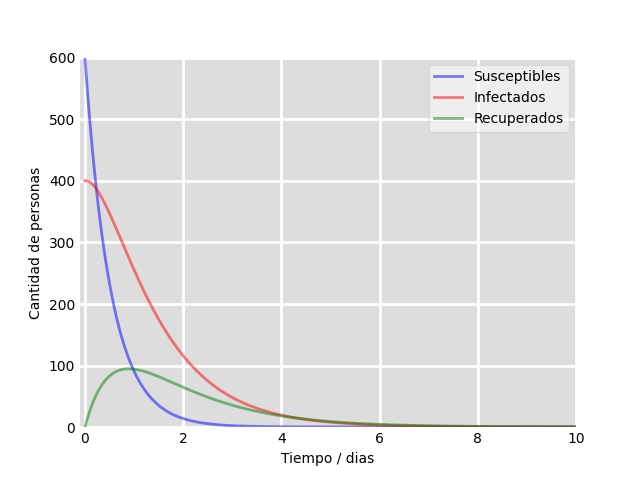
\includegraphics[width=1\textwidth]{./images/Figure_1.png}
    \caption{Gr\'afica del modelo SIR}
    \label{fig:model_graph}
\end{figure}

Podemos obvervar un comportamiento inusual ya que se  reduce la cantidad de recuperados con el paso del tiempo. Esto se puede deber a un error en el art\'iculo, en nuestra interpretaci\'on de este, o en la selecci\'on de los par\'ametros. Los par\'ametros usados fueron los mismos que en el cuadro \ref{tab:r_0_comparison}, adem\'as de los valores $\rho=0.6$, $a=0.2$, $b=0.4$, $\gamma=0.003$, y las condiciones iniciales $S(0)=600$, $I(0)=400$, $R(0)=0$.

\section{Puntos de Equilibrio, Diagrama de Fase y Estabilidad del sistema}

Para analizar la estabilidad del sistema necesitamos reducir nuestro modelo, ya que este cuenta con 3 ecuaciones. 

Para ello tenemos que: ${dN\over dt}=\alpha-\beta N$, de donde el único punto de equilibrio es $\alpha-\beta N=0\Rightarrow N(t)={\alpha\over\beta}\Rightarrow S+R+I={\alpha\over\beta}$. De este razonamiento y de nuestro sistema \textbf{SIR} obtenemos el siguiente sistema reducido:

\begin{equation}
	{dI\over dt}={kI\rho (1+aI)\over 1+bI^2}\Big({\alpha\over\beta}-I-R\Big)-(\beta+\mu)I
\end{equation}

\begin{equation}
	{dR\over dt}=\mu I-(\beta+\gamma)R+{kI(1+aI)(1-\rho)\over 1+bI^2}\Big({\alpha\over\beta}-I-R\Big)
\end{equation}

Ahora tratemos de buscar un sistema equivalente m\'as c\'omodo para realizar el an\'alisis de estabilidad, para ello sea $x={k\over \beta +\gamma}I$, $y={k\over \beta +\gamma}R$ y $\tau = (\beta+\gamma)t$, donde $A={\alpha k\over \beta(\beta+\gamma)}$, $p={a(\beta+\gamma)\over k}$, $q={b(\beta+\gamma)^2\over k^2}$, $B=\rho$, $m={\beta+\mu\over \beta+\gamma}$ y $r={\mu\over \beta+\gamma}$, entonces:

\begin{equation}
	{dx\over d\tau}={x(1+px)B\over 1+qx^2}(A-x-y)-mx
\end{equation}

\begin{equation}
	{dy\over d\tau}=rx-y+{1+px\over 1+qx^2}(1-B)x(A-x-y)
\end{equation}

Ahora analicemos el siguiente diagrama de fase que describe el sistema anterior:

\begin{figure}[H]
    \centering
    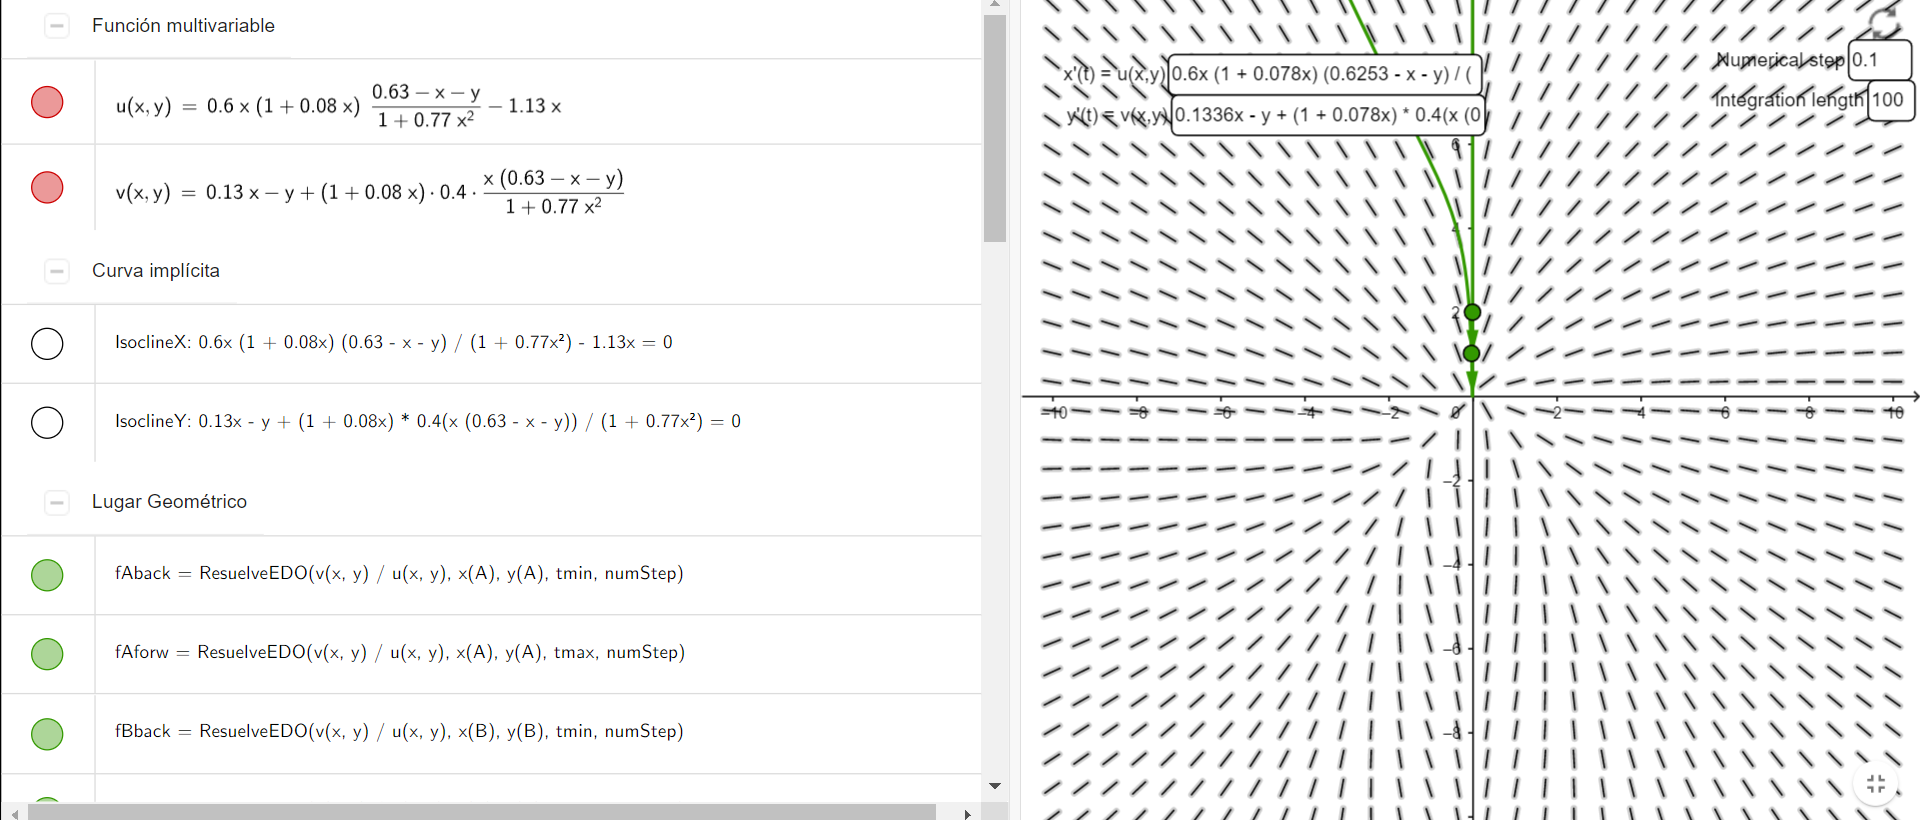
\includegraphics[width=1\textwidth]{./images/Figure_2.png}
    \caption{Diagrama de Fase}
    \label{fig:phase_diagram}
\end{figure}

Aqu\'i podemos observar que existe un \'unico punto de equilibrio en el sistema en el punto (0,0). El cual se alcanza con las siguientes soluciones: $$x^*={By\over m+B(r-m)}$$ $$y^*={(m+B(r-m)x^*\over B}$$

Analicemos la matriz Jacobiana del sistema formado por las ecuaciones (13) y (14), teniendo en cuenta que $D = \dfrac{(1+bI^2)}{(1+aI)\rho kI}$:

\begin{equation}
	M=\left(
	\begin{matrix}
		 BD-m & -{B(1+px)x\over 1+qx^2}\\
		 r+(1-B)D & -1-{(1-B)(1+px)x\over 1+qx^2}
	\end{matrix}
	\right)
\end{equation}

Ahora si se cumple que:

\begin{equation}
m+{m(1-B)(1+px)x\over 1+qx^2}+{rB(1+px)x\over 1+qx^2}>BD
\end{equation}

entonces tenemos que ($x^*$,$y^*$) es un nodo o un foco o un centro del sistema.

\begin{equation}
	tr(M)=BD-m-1-{(1-B)(1+px)x\over 1+qx^2}
\end{equation}

Si $m+1+{(1-B)(1+px)x\over 1+qx^2}>BD$ entonces $tr(M)<0$, donde:
$$D={(1+qx^2)(A-x-y)(1+2px)-(x+px^2)(1+qx^2+(A-x-y)2px)\over 1+qx^2}$$

Por tanto las condiciones de las ecuaciones (16) y (17) son satisfacidas, luego existe un \'unico punto de equilibrio en el sistema, (0,0), el cual podemos decir que es estable. 
	
\section{Conclusiones}

Durante el desarrollo de este trabajo pudimos adquirir conocimientos sobre el funcionamiento del modelo SIR, el cual resulta ser muy empleado en la modelaci\'on de la propagación de enfermedades infecciosas. Adem\'as descubrimos herramientas \'utiles para determinar los puntos de equilibrio de un sistema de ecuaciones diferenciales, y como estos puntos afectan el comportamiento del sistema. Tambi\'en aprendimos sobre la  metodolog\'ia que se emplea para analizar la estabilidad del sistema en dichos puntos mediante la experimentaci\'on con esta. \par
Creemos habernos topado con algunos errores en el art\'iculo estudiado. El primer ejemplo de esto fue la discrepancia entre los valores de $R_0$ para diferentes valores de $\rho$ entre el art\'iculo y nuestra experimentaci\'on. Tambi\'en debemos hacer notar el comportamiento inusual del valor $R$, pues como podemos ver en la figura \ref{fig:model_graph}, a partir de cierto punto la cantidad de recuperados se reduce, cosa que no deber\'ia suceder en un modelo SIR. Intentamos modificar las constantes del modelo para ver si esto se solucionaba, pero no tuvimos \'exito. \par
Teniendo en cuenta lo anterior creemos conveniente recomendar una revisi\'on m\'as exhaustiva del modelo propuesto en el art\'iculo, para ver si se puede corregir el error que se presenta en el mismo. \par


\section{Bibliograf\'ia}

\begin{enumerate}
    \item Ecuaciones diferenciales y problemas con valores en la frontera; Edwards, C. Henry; Pearson Education; 2001
    \item Differential equations and dynamical systems; Perko, Lawrence; Springer, 2001
    \item Stability analysis of an SIR model with immunity and modified transmission function; Nidhi Nirwani et al.; International Journal of Applied Mathematical Research; 2015
\end{enumerate}

\section{Anexos}

\subsection*{Anexo 1: Graficado del sistema de EDO del modelo SIR}

\begin{lstlisting}[label={lst:runge_kutta}]

# Metodo de Runge-Kutta de 4to orden
def rk4(f, x, t, h, N, beta, gamma, alpha, k, miu, ro, a, b):
    k1 = h * f(x, t, N, beta, gamma, alpha, k, miu, ro, a, b)
    k2 = h * f(x + 0.5 * k1, t + 0.5 * h, N, beta, gamma, alpha, k, miu, ro, a, b)
    k3 = h * f(x + 0.5 * k2, t + 0.5 * h, N, beta, gamma, alpha, k, miu, ro, a, b)
    k4 = h * f(x + k3, t + h, N, beta, gamma, alpha, k, miu, ro, a, b)
    return x + (k1 + 2 * k2 + 2 * k3 + k4) / 6

# Sistema de ecuaciones diferenciales del modelo
def deriv(y, t, N, beta, gamma, alpha, k, miu, ro, a, b):
    S, I, R = y
    dSdt = alpha - beta * S - ((1 + a * I) * k * I * S) / (1 + b * I ** 2) + gamma * R
    dIdt = ((1 + a * I) * ro * k * I * S) / (1 + b * I ** 2) - (beta + miu) * I
    dRdt = miu * I - (beta + gamma) * R + ((1 + a * I) * (1 - ro) * k * I * S) / (1 + b * I ** 2)
    return np.array([dSdt, dIdt, dRdt])


t = np.linspace(0, 10, 200)    
# Vector de condiciones iniciales
y0 = np.array([S0, I0, R0])
# Aproximar las ecuaciones del modelo con el metodo de Runge-Kutta de 4to orden
ret = np.array([y0])
for i in range(len(t) - 1):
    ret = np.vstack((ret, rk4(deriv, ret[-1], t[i], t[i + 1] - t[i], N, beta, gamma, alpha, k, miu, ro, a, b)))
S, I, R = ret.T

\end{lstlisting}

\end{document}